%%%%%%%%%%%%%%%%%%%%%%%%%%%%%%%%%%%%%%%%%%%%%%%%%%%%%%%%%%%%%%%%%%%%%%%%%%%%%%%%
\documentclass[11pt]{article} % Dokumentenklasse

\usepackage[utf8]{inputenc} % Textkodierung: UTF-8
\usepackage[T1]{fontenc} % Zeichensatzkodierung

\usepackage[USenglish]{babel}% http://ctan.org/pkg/babel
\usepackage{graphicx} % Grafiken
\usepackage[absolute]{textpos} % Positionierung

% Schriftart Helvetica:
\usepackage[scaled]{helvet}
\renewcommand{\familydefault}{\sfdefault}

\usepackage{calc} % Berechnungen
\usepackage{tabto} % Tabulatoren
\usepackage{parskip}

\usepackage{enumitem}

% Debugging:
%\usepackage{layout} % Layout-Informationen
%\usepackage{printlen} % Längenwerte ausgeben

%%%%%%%%%%%%%%%%%%%%%%%%%%%%%%%%%%%%%%%%%%%%%%%%%%%%%%%%%%%%%%%%%%%%%%%%%%%%%%%%
% EINSTELLUNGEN
%%%%%%%%%%%%%%%%%%%%%%%%%%%%%%%%%%%%%%%%%%%%%%%%%%%%%%%%%%%%%%%%%%%%%%%%%%%%%%%%

% Seitenränder:
\newcommand{\SeitenrandOben}{43.5mm}
\newcommand{\SeitenrandRechts}{20mm}
\newcommand{\SeitenrandLinks}{20mm}
\newcommand{\SeitenrandUnten}{10mm}

\newcommand{\UniversitaetLogoBreite}{19mm}
\newcommand{\UniversitaetLogoHoehe}{1cm}

\usepackage[a4paper,
top=\SeitenrandOben,
bottom=\SeitenrandUnten,
inner=\SeitenrandLinks,
outer=\SeitenrandRechts,
foot=0cm,
head=0cm
]{geometry}

\textblockorigin{\SeitenrandLinks}{\SeitenrandOben} % Ursprung für Positionierung

\setlength{\parindent}{0pt}
%\setlength{\baselineskip}{32pt}
\setlength{\parskip}{\baselineskip}
\TabPositions{4cm}
\pagestyle{empty}

%%%%%%%%%%%%%%%%%%%%%%%%%%%%%%%%%%%%%%%%%%%%%%%%%%%%%%%%%%%%%%%%%%%%%%%%%%%%%%%%
% General stuff
%%%%%%%%%%%%%%%%%%%%%%%%%%%%%%%%%%%%%%%%%%%%%%%%%%%%%%%%%%%%%%%%%%%%%%%%%%%%%%%%
\newcommand{\Problem}[1]{\paragraph*{Problem #1:}\qquad}
\newcommand{\Topic}[1]{
	\newpage
	\section*{#1}}

\newcommand{\Given}{\textbf{Given:\qquad\qquad}}
\newcommand{\Searched}{\textbf{Searched:\qquad}}
\newcommand{\Solution}{\textbf{Solution:\qquad}}

%%%%%%%%%%%%%%%%%%%%%%%%%%%%%%%%%%%%%%%%%%%%%%%%%%%%%%%%%%%%%%%%%%%%%%%%%%%%%%%%
% Math stuff
%%%%%%%%%%%%%%%%%%%%%%%%%%%%%%%%%%%%%%%%%%%%%%%%%%%%%%%%%%%%%%%%%%%%%%%%%%%%%%%%
\usepackage{amsmath}
\usepackage{amssymb}

\newcommand{\R}{\mathbb{R}}
\newcommand{\Vector}[1]{\R^{#1}}
\newcommand{\Matrix}[2]{\R^{#1 \times #2}} % !!! DON'T TOUCH !!!
%%%%%%%%%%%%%%%%%%%%%%%%%%%%%%%%%%%%%%%%%%%%%%%%%%%%%%%%%%%%%%%%%%%%%%%%%%%%%%%%


\newcommand{\ExerciseNumber}{04}

\newcommand{\PersonOne}{Marcel Bruckner (03674122)}
\newcommand{\PersonTwo}{Julian Hohenadel (03673879)}
\newcommand{\PersonThree}{Kevin Bein (03707775)}

%%%%%%%%%%%%%%%%%%%%%%%%%%%%%%%%%%%%%%%%%%%%%%%%%%%%%%%%%%%%%%%%%%%%%%%%%%%%%%%%
% DOKUMENT
%%%%%%%%%%%%%%%%%%%%%%%%%%%%%%%%%%%%%%%%%%%%%%%%%%%%%%%%%%%%%%%%%%%%%%%%%%%%%%%%

\begin{document}

%%%%%%%%%%%%%%%%%%%%%%%%%%%%%%%%%%%%%%%%%%%%%%%%%%%%%%%%%%%%%%%%%%%%%%%%%%%%%%%%
\begin{textblock*}{\UniversitaetLogoBreite}[1,0](\textwidth-1mm, 2cm-\SeitenrandOben)%
	\raggedleft
\includegraphics{../Ressources/Universitaet_Logo_RGB.pdf}%
\end{textblock*}


\begin{textblock*}{\textwidth}[0,0](0cm, 0cm)%
	{\fontsize{24pt}{26pt}\selectfont\textbf{Exercise}}
	
	\vspace*{14pt}
	{\fontsize{18pt}{27pt}\selectfont\textbf{\ExerciseNumber}}
\end{textblock*}

\vspace*{92.2mm}
\fontsize{15pt}{17.5pt}\selectfont%
TUM Department of Informatics

\renewcommand{\baselinestretch}{1.47}
\normalsize\selectfont
\vspace*{17.1mm}
\textbf{Supervised by}\tab
\begin{minipage}[t]{\textwidth-\CurrentLineWidth}
	Prof. Dr. Stephan Günnemann\\
	Informatics 3 - Professorship of Data Mining and Analytics\strut
\end{minipage}

\vspace*{4.3mm}
\textbf{Submitted by}\tab
\begin{minipage}[t]{\textwidth-\CurrentLineWidth}
	\PersonOne\\
	\PersonTwo\\
	\PersonThree
\end{minipage}

\vspace*{-1mm}
\textbf{Submission date}\tab 
\begin{minipage}[t]{\textwidth-\CurrentLineWidth}
	Munich, \today
\end{minipage}
\newpage % !!! DON'T TOUCH !!!
%%%%%%%%%%%%%%%%%%%%%%%%%%%%%%%%%%%%%%%%%%%%%%%%%%%%%%%%%%%%%%%%%%%%%%%%%%%%%%%%

%%%%%%%%%%%%%%%%%%%%%%%%%%%%%%%%%%%%%%%%%%%%%%%%%%%%%%%%%%%%%%%%%%%%%%%%%%%%%%%%
% !!! HOMEWORK STARTS HERE !!!
%%%%%%%%%%%%%%%%%%%%%%%%%%%%%%%%%%%%%%%%%%%%%%%%%%%%%%%%%%%%%%%%%%%%%%%%%%%%%%%%
%
\Topic{Least squares regression}
%
\Problem{1}
%
\begin{flushleft}
Using $T = diag(t_i)$, the derivative can be calculated similar to the lecture:
\end{flushleft}
\begin{align*}
  \nabla_w E_\text{weighted}(w) &= \nabla_w \frac{1}{2} \sum_{i=1}^N t_i \left[w^T \phi(x_i) - y_i\right]^2 \\
  &= \nabla_w \frac{1}{2} (\Phi w - y)^T T (\Phi w - y) \\
  &= \nabla_w \frac{1}{2} (w^T \Phi^T - y^T)(T\Phi w - T y) \\
  &= \nabla_w \frac{1}{2} (w^T \Phi^T T \Phi w - 2w^T \Phi^T T y + y^T T y) \\
  &= \nabla_w (\frac{1}{2} w^T \Phi^T T \Phi w - w^T \Phi^T T y + \frac{1}{2}y^T T y) \\
  &= \Phi^T T \Phi w - \Phi^T T y \\
  &\overset{!}{=} 0
  & \\
  &\Rightarrow \Phi^T T y = \Phi^T T \Phi w \\
  &\Rightarrow w = \Phi^T T y (\Phi^T T \Phi)^{-1} 
\end{align*}
%
\textit{Missing explanation for 1) and 2)}
%
%
\Topic{Ridge regression}
%
\Problem{2}
%
\begin{align*}
  E_\text{LS} &= \frac{1}{2} \sum_{i=1}^N \left[w^T \phi(x_i) - y_i\right]^2 \\
  &= \frac{1}{2} (\Phi w - y)^T (\Phi w - y) \\
  E_\text{ridge} &= \frac{1}{2} \sum_{i=1}^N \left[w^T \phi(x_i) - y_i\right]^2 + \frac{\lambda}{2} ||w||_2^2 \\
  &= \frac{1}{2} (\Phi w - y)^T (\Phi w - y) + \frac{\lambda}{2} ||w||_2^2 
\end{align*}
\begin{flushleft}
Following the instructions, we can augment the design matrix $\Phi$ and $y$:
\end{flushleft}
\begin{align*}
\Phi &= 
\begin{pmatrix}
  \phi_1(x_1) & \ldots & \phi_M(x_1) \\
  \vdots & \ddots & \vdots \\
  \phi_1(x_N) & \ldots & \phi_M(x_N)
\end{pmatrix} \in \mathbb{R}^{N \times M} \\
\Rightarrow \Phi_A &=
\begin{pmatrix}
  \phi_1(x_1) & \ldots & \phi_M(x_1) \\
  \vdots & \ddots & \vdots \\
  \phi_1(x_N) & \ldots & \phi_M(x_N) \\
  \sqrt{\lambda} I & & 0 \\
  & \ddots & \\
  0 & & \sqrt{\lambda} I
\end{pmatrix} =
\begin{pmatrix} \Phi \\ \sqrt{\lambda} I \end{pmatrix}
\in \mathbb{R}^{N \times M+M} 
\end{align*}
\begin{align*}
  y &= \begin{pmatrix} y_1 \\ \vdots \\ y_M \end{pmatrix}
  \in \mathbb{R}^M 
  \Rightarrow y_A = \begin{pmatrix} y_1 \\ \vdots \\ y_M \\ 0_1 \\ \vdots \\ 0_M \end{pmatrix}
  = \begin{pmatrix} y \\ 0 \end{pmatrix}
\in \mathbb{R}^{M+M}
\end{align*}
\begin{flushleft}
Inserting $\Phi_A$ and $y_A$ into $E_\text{LS}(w)$ directly gives ridge regression:
\begin{align*}
  E_\text{LS}(w) &= \frac{1}{2} (\Phi_A w - y_A)^T (\Phi_A w - y_A) = \frac{1}{2} (\Phi w - y)^T (\Phi w - y) + \frac{\lambda}{2} ||w||_2^2 = E_\text{ridge}(w) \\
\end{align*}
\end{flushleft}
%
\newpage
\Problem{3}
%
\begin{align*}
\nabla_w E_\text{ridge}(w) &= \nabla_w \left[\frac{1}{2} (\Phi w - y)^T (\Phi w - y) + \frac{\lambda}{2} ||w||^2_2 \right] \\
&= \nabla_w \frac{1}{2} (\Phi w - y)^T (\Phi w - y) + \nabla_w \frac{\lambda}{2} ||w||^2_2 \\
&= (\Phi^T \Phi w - \Phi^T y) + \lambda w \\
&\overset{!}{=} 0 \\
&\Rightarrow \Phi^T\Phi w - \Phi^T y + \lambda w = 0 \\
&\Rightarrow \Phi^T\Phi w  + \lambda w = \Phi^T y \\
&\Rightarrow (\Phi^T \Phi + \lambda I) w = \Phi^T y \\
&\Rightarrow w = (\Phi^T \Phi + \lambda I)^{-1} \Phi^T y
\end{align*}
\begin{flushleft}
  When $N < M$ then the covariance Matrix $\Phi^T \Phi$ becomes singular ($det(\Phi^T\Phi) = 0)$ and thus cannot be inverted anymore. Adding the L2-Regularization term in ridge regression $\Phi^T \Phi + \lambda I$ fixes this problem and the inverse can be computed again. L2 also increases the numerical stability by reducing the variance of the matrix and thus roundoff errors cannot accumulate as fast.
\end{flushleft}
%
\Topic{Multi-output linear regression}
%
\Problem{4}
%
%
\Topic{Comparison of linear regression models}
%
\Problem{5}
%
%
\Topic{Programming Task}
%
\Problem{6}
%
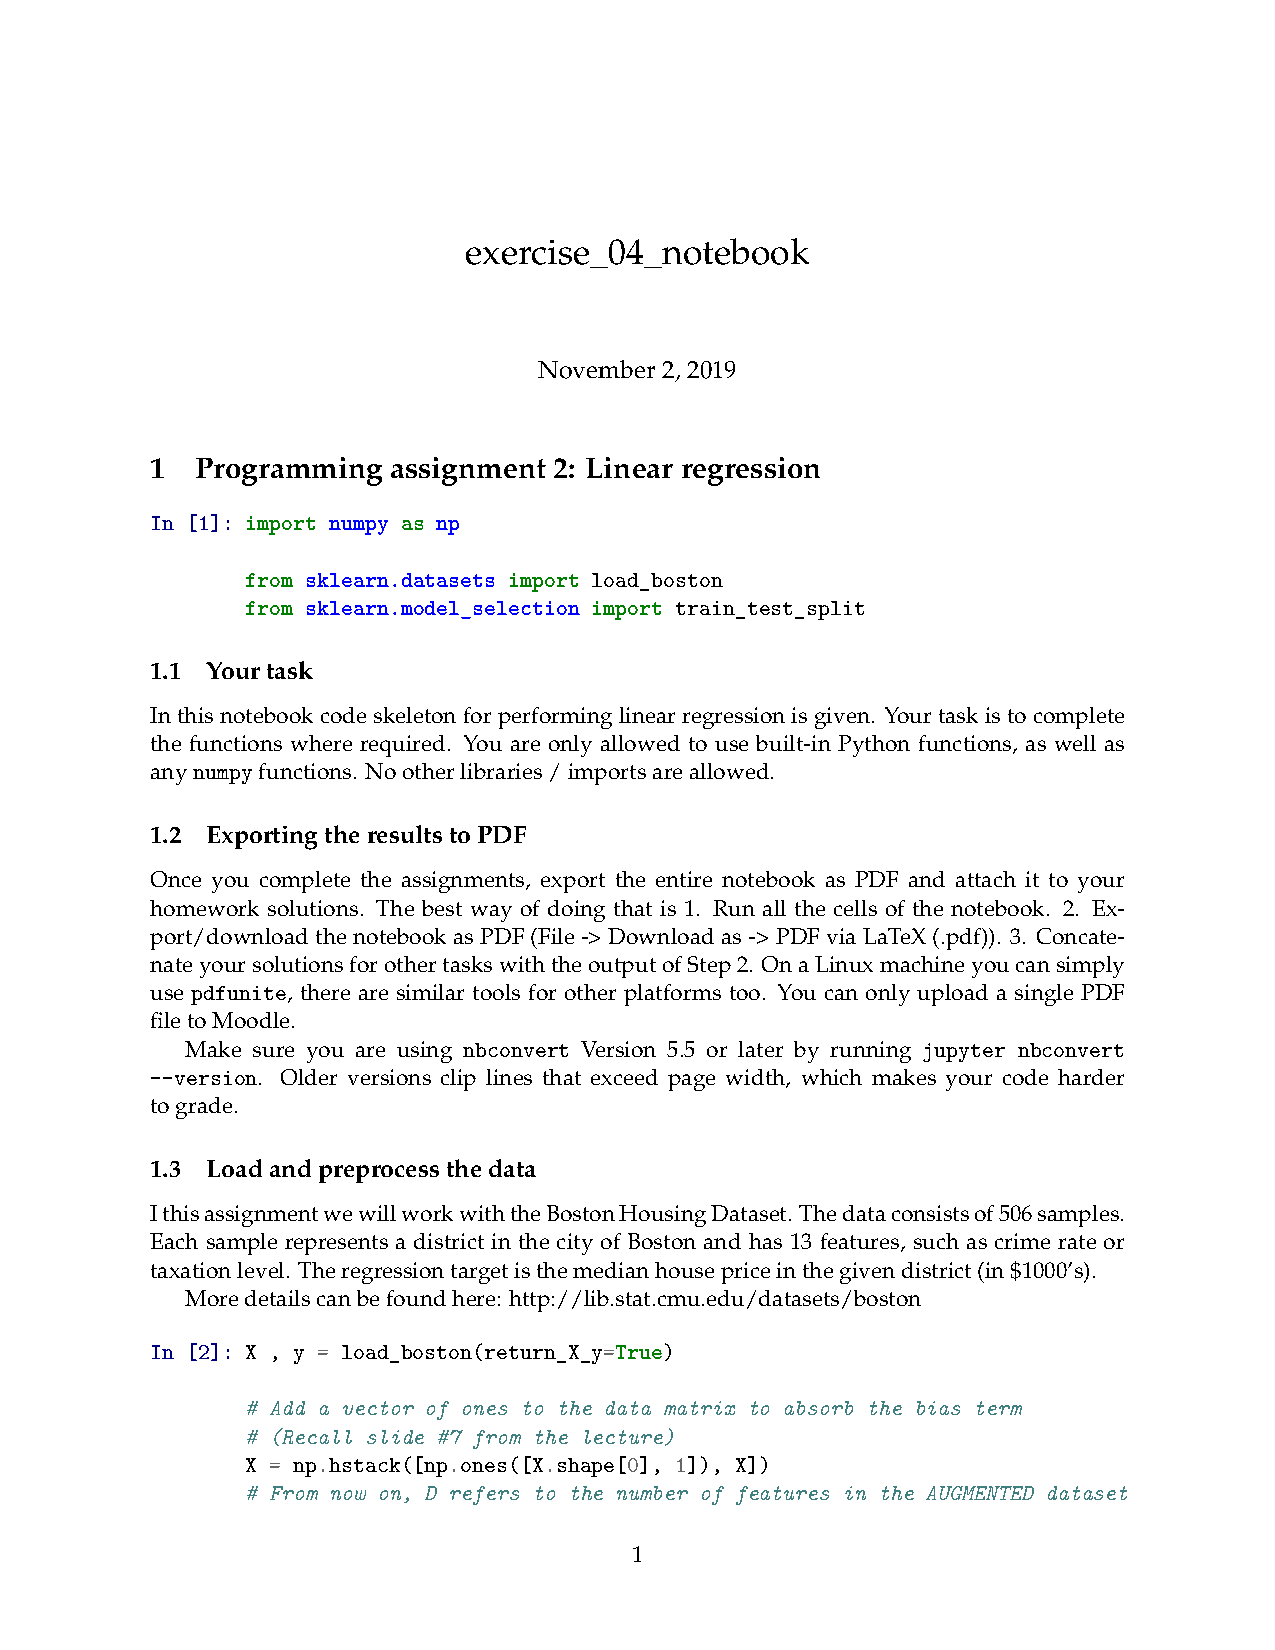
\includepdf[pages=-]{exercise_04_notebook.pdf}
%
%%%%%%%%%%%%%%%%%%%%%%%%%%%%%%%%%%%%%%%%%%%%%%%%%%%%%%%%%%%%%%%%%%%%%%%%%%%%%%%%
% !!! HOMEWORK ENDS HERE !!!
%%%%%%%%%%%%%%%%%%%%%%%%%%%%%%%%%%%%%%%%%%%%%%%%%%%%%%%%%%%%%%%%%%%%%%%%%%%%%%%%

%%%%%%%%%%%%%%%%%%%%%%%%%%%%%%%%%%%%%%%%%%%%%%%%%%%%%%%%%%%%%%%%%%%%%%%%%%%%%%%%
\newpage

\vspace*{-15.8mm}
\fontsize{19pt}{21pt}\selectfont

\vspace{25.3mm}
Appendix

\normalsize\selectfont
\vspace{13.2mm}
We confirm that the submitted solution is original work and was written by us without further assistance. Appropriate credit has been given where reference has been made to the work of others.

\vspace{18.1mm}
\rule[-3.7mm]{\linewidth}{0.5pt}
Munich, \today, Signature \PersonOne

\vspace{18.1mm}
\rule[-3.7mm]{\linewidth}{0.5pt}
Munich, \today, Signature \PersonTwo

\vspace{18.1mm}
\rule[-3.7mm]{\linewidth}{0.5pt}
Munich, \today, Signature \PersonThree
 % !!! DON'T TOUCH !!!
%%%%%%%%%%%%%%%%%%%%%%%%%%%%%%%%%%%%%%%%%%%%%%%%%%%%%%%%%%%%%%%%%%%%%%%%%%%%%%%%

\end{document}
